\documentclass[journal,12pt,twocolumn]{IEEEtran}

\usepackage{setspace}
\usepackage{gensymb}
\singlespacing
\usepackage[cmex10]{amsmath}

\usepackage{amsthm}

\usepackage{mathrsfs}
\usepackage{txfonts}
\usepackage{stfloats}
\usepackage{bm}
\usepackage{tcolorbox}
\usepackage{cite}
\usepackage{cases}
\usepackage{subfig}
\usepackage[T1]{fontenc}
\usepackage{inconsolata}

\usepackage{longtable}
\usepackage{multirow}
\usepackage{amsmath}

\usepackage{enumitem}
\usepackage{mathtools}
\usepackage{steinmetz}
\usepackage{tikz}
\usepackage{circuitikz}
\usepackage{verbatim}
\usepackage{tfrupee}
\usepackage[breaklinks=true]{hyperref}
\usepackage{graphicx}
\usepackage{tkz-euclide}
\usetikzlibrary{positioning}

\usetikzlibrary{calc,math}
\usepackage{listings}
    \usepackage{color}                                            %%
    \usepackage{array}                                            %%
    \usepackage{longtable}                                        %%
    \usepackage{calc}                                             %%
    \usepackage{multirow}                                         %%
    \usepackage{hhline}                                           %%
    \usepackage{ifthen}                                           %%
    \usepackage{lscape}     
\usepackage{multicol}
\usepackage{chngcntr}

\DeclareMathOperator*{\Res}{Res}

\renewcommand\thesection{\arabic{section}}
\renewcommand\thesubsection{\thesection.\arabic{subsection}}
\renewcommand\thesubsubsection{\thesubsection.\arabic{subsubsection}}

\renewcommand\thesectiondis{\arabic{section}}
\renewcommand\thesubsectiondis{\thesectiondis.\arabic{subsection}}
\renewcommand\thesubsubsectiondis{\thesubsectiondis.\arabic{subsubsection}}


\hyphenation{op-tical net-works semi-conduc-tor}
\def\inputGnumericTable{}                                 %%

\lstset{
%language=C,
frame=single, 
breaklines=true,
columns=fullflexible
}
\begin{document}


\newtheorem{theorem}{Theorem}[section]
\newtheorem{problem}{Problem}
\newtheorem{proposition}{Proposition}[section]
\newtheorem{lemma}{Lemma}[section]
\newtheorem{corollary}[theorem]{Corollary}
\newtheorem{example}{Example}[section]
\newtheorem{definition}[problem]{Definition}

\newcommand{\BEQA}{\begin{eqnarray}}
\newcommand{\EEQA}{\end{eqnarray}}
\newcommand{\define}{\stackrel{\triangle}{=}}
\bibliographystyle{IEEEtran}
\raggedbottom
\setlength{\parindent}{0pt}
\providecommand{\mbf}{\mathbf}
\providecommand{\pr}[1]{\ensuremath{\Pr\left(#1\right)}}
\providecommand{\qfunc}[1]{\ensuremath{Q\left(#1\right)}}
\providecommand{\sbrak}[1]{\ensuremath{{}\left[#1\right]}}
\providecommand{\lsbrak}[1]{\ensuremath{{}\left[#1\right.}}
\providecommand{\rsbrak}[1]{\ensuremath{{}\left.#1\right]}}
\providecommand{\brak}[1]{\ensuremath{\left(#1\right)}}
\providecommand{\lbrak}[1]{\ensuremath{\left(#1\right.}}
\providecommand{\rbrak}[1]{\ensuremath{\left.#1\right)}}
\providecommand{\cbrak}[1]{\ensuremath{\left\{#1\right\}}}
\providecommand{\lcbrak}[1]{\ensuremath{\left\{#1\right.}}
\providecommand{\rcbrak}[1]{\ensuremath{\left.#1\right\}}}
\theoremstyle{remark}
\newtheorem{rem}{Remark}
\newcommand{\sgn}{\mathop{\mathrm{sgn}}}
\providecommand{\abs}[1]{\left\vert#1\right\vert}
\providecommand{\res}[1]{\Res\displaylimits_{#1}} 
\providecommand{\norm}[1]{\left\lVert#1\right\rVert}
%\providecommand{\norm}[1]{\lVert#1\rVert}
\providecommand{\mtx}[1]{\mathbf{#1}}
\providecommand{\mean}[1]{E\left[ #1 \right]}
\providecommand{\fourier}{\overset{\mathcal{F}}{ \rightleftharpoons}}
%\providecommand{\hilbert}{\overset{\mathcal{H}}{ \rightleftharpoons}}
\providecommand{\system}{\overset{\mathcal{H}}{ \longleftrightarrow}}
	%\newcommand{\solution}[2]{\textbf{Solution:}{#1}}
\newcommand{\solution}{\noindent \textbf{Solution: }}
\newcommand{\cosec}{\,\text{cosec}\,}
\providecommand{\dec}[2]{\ensuremath{\overset{#1}{\underset{#2}{\gtrless}}}}
\newcommand{\myvec}[1]{\ensuremath{\begin{pmatrix}#1\end{pmatrix}}}
\newcommand{\mydet}[1]{\ensuremath{\begin{vmatrix}#1\end{vmatrix}}}
\numberwithin{equation}{subsection}
\makeatletter
\@addtoreset{figure}{problem}
\makeatother
\let\StandardTheFigure\thefigure
\let\vec\mathbf
\renewcommand{\thefigure}{\theproblem}
\def\putbox#1#2#3{\makebox[0in][l]{\makebox[#1][l]{}\raisebox{\baselineskip}[0in][0in]{\raisebox{#2}[0in][0in]{#3}}}}
     \def\rightbox#1{\makebox[0in][r]{#1}}
     \def\centbox#1{\makebox[0in]{#1}}
     \def\topbox#1{\raisebox{-\baselineskip}[0in][0in]{#1}}
     \def\midbox#1{\raisebox{-0.5\baselineskip}[0in][0in]{#1}}
\vspace{3cm}
\title{Assignment-1}
\author{Adithya Vardhan - EE18BTECH11008}
\maketitle
\newpage
\bigskip
\renewcommand{\thefigure}{\theenumi}
\renewcommand{\thetable}{\theenumi}
Github repository
\begin{lstlisting}
https://github.com/Adithya-Vardhan/GVV_C-DS
\end{lstlisting}
%
\section{\textbf{Problem}}
\textbf{Consider the following two functions:}
\begin{tcolorbox}
\begin{verbatim}
void fun1(int n) {
    if (n==0) return;
    printf("%d",n);
    fun2(n-2);
    printf("%d",n);
}
void fun2(int n) {
    if (n==0) return;
    printf("%d",n);
    fun1(++n);
    printf("%d",n);
}
\end{verbatim}
\end{tcolorbox}
The output printed when fun1(5) is called is \_.
\section{\textbf{Solution}}
\textbf{Answer:} Option 1. 53423122233445
\\~\\
Given two functions will terminate when the input "n" is equal to zero.
\\~\\ 
Whenever we execute fun1(n), it will invoke fun2(n-2), if n is not equal to zero and there will be no change in the value in the value of n, before and after execution of fun2(n-2). So fun1(n) will print same n before and after execution of fun2(n-2).
\\~\\ 
But when we execute fun2(n), it will invoke fun1(++n),if n is not equal to zero. Lets say n is input-integer.So after the execution of fun1(++n), n will be assigned to input-integer+1. There will be a increment of 1 in n after execution of fun1(++n) when compared to n before execution of fun1(++n). So fun2(n) will print n before execution of fun1(++n) and n+1 after execution of fun1(++n).
\\~\\
\begin{center}
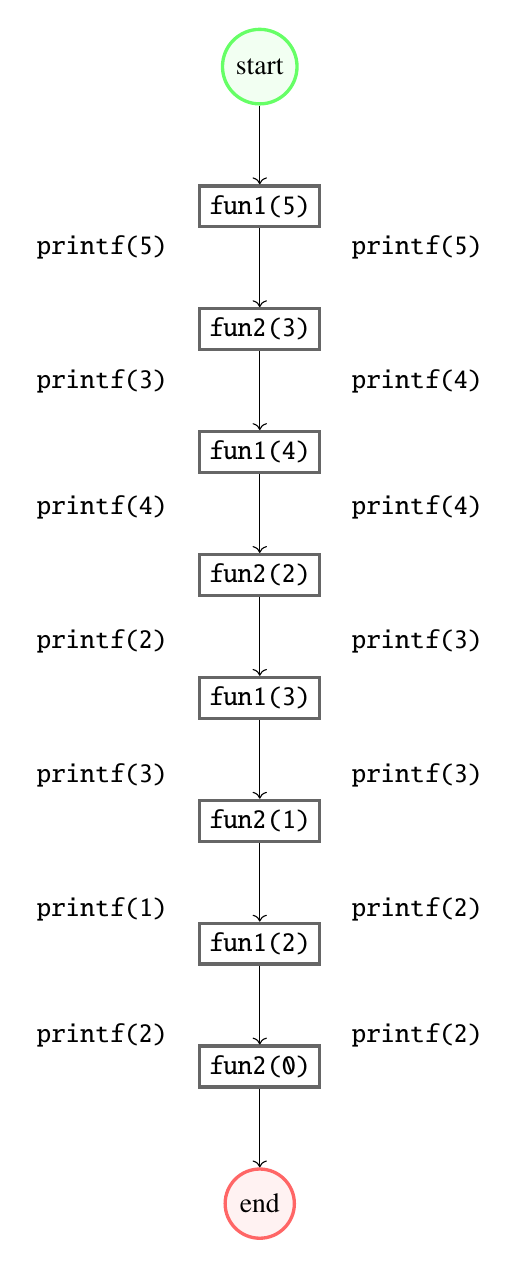
\begin{tikzpicture}[
roundnode/.style={circle, draw=green!60, fill=green!5, very thick, minimum size=7mm},
round2node/.style={circle, draw=red!60, fill=red!5, very thick, minimum size=7mm},
squarednode/.style={rectangle, draw=black!60, fill=white!5, very thick, minimum size=5mm},
]
%Nodes
\node[roundnode]        (start)                                 {start};
\node[squarednode]      (first)        [below=of start]         {\texttt{fun1(5)}};
\node[squarednode]      (second)       [below=of first]         {\texttt{fun2(3)}};
\node[squarednode]      (third)        [below=of second]        {\texttt{fun1(4)}};
\node[squarednode]      (fourth)       [below=of third]         {\texttt{fun2(2)}};
\node[squarednode]      (fifth)       [below=of fourth]         {\texttt{fun1(3)}};
\node[squarednode]      (sixth)       [below=of fifth]         
{\texttt{fun2(1)}};
\node[squarednode]      (seventh)       [below=of sixth]         {\texttt{fun1(2)}};
\node[squarednode]      (eigth)       [below=of seventh]         {\texttt{fun2(0)}};
\node[round2node]        (end)          [below=of eigth]     {end};
%Lines
\draw[->] (start.south) -- (first.north);
\draw[->] (first.south) -- (second.north);
\draw[->] (second.south) -- (third.north);
\draw[->] (third.south) -- (fourth.north);
\draw[->] (fourth.south) -- (fifth.north);
\draw[->] (fifth.south) -- (sixth.north);
\draw[->] (sixth.south) -- (seventh.north);
\draw[->] (seventh.south) -- (eigth.north);
\draw[->] (eigth.south) -- (end.north);
%Text
\node[] at (-2,-2.3) {\texttt{printf(5)}};
\node[] at (2,-2.3) {\texttt{printf(5)}};
\node[] at (-2,-4.0) {\texttt{printf(3)}};
\node[] at (2,-4.0) {\texttt{printf(4)}};
\node[] at (-2,-5.6) {\texttt{printf(4)}};
\node[] at (2,-5.6) {\texttt{printf(4)}};
\node[] at (-2,-7.3) {\texttt{printf(2)}};
\node[] at (2,-7.3) {\texttt{printf(3)}};
\node[] at (-2,-9.0) {\texttt{printf(3)}};
\node[] at (2,-9.0) {\texttt{printf(3)}};
\node[] at (-2,-10.7) {\texttt{printf(1)}};
\node[] at (2,-10.7) {\texttt{printf(2)}};
\node[] at (-2,-12.3) {\texttt{printf(2)}};
\node[] at (2,-12.3) {\texttt{printf(2)}};


\end{tikzpicture}

\end{document}
